\documentclass[a4paper,12pt]{article}
\usepackage[margin=18mm]{geometry}
\usepackage{tikz}
\usepackage{amsmath}
\newcommand{\pFourCell}[1]{\makebox[1.75em][c]{\ensuremath{#1}}}
\pagestyle{empty}
\begin{document}
\section*{Spaltentreue LaTeX-Ausgabe}
\noindent Gleichung: \texttt{2*sqrt((x+3)/(2+1))=5} \hfill Zielvariable: \texttt{x}

\vspace{8mm}
\begin{center}
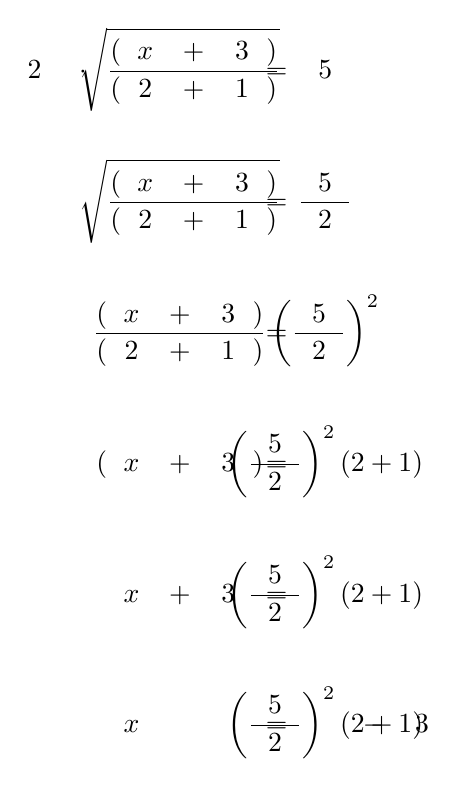
\begin{tikzpicture}[x=1.75em,y=-1em]
\node[anchor=base, inner sep=0pt] at (3,2.9) {$2$};
\node[anchor=base, inner sep=0pt] at (4,2.9) {$\cdot$};
\node[anchor=base, inner sep=0pt] at (6,2.9) {$\sqrt{\displaystyle\frac{\left(\pFourCell{x}\pFourCell{+}\pFourCell{3}\right)}{\left(\pFourCell{2}\pFourCell{+}\pFourCell{1}\right)}}$};
\node[anchor=base, inner sep=0pt] at (8,2.9) {$=$};
\node[anchor=base, inner sep=0pt] at (9,2.9) {$5$};
\node[anchor=base, inner sep=0pt] at (9,7.6499999999999995) {$\displaystyle\frac{\pFourCell{5}}{\pFourCell{2}}$};
\node[anchor=base, inner sep=0pt] at (6,7.6499999999999995) {$\sqrt{\displaystyle\frac{\left(\pFourCell{x}\pFourCell{+}\pFourCell{3}\right)}{\left(\pFourCell{2}\pFourCell{+}\pFourCell{1}\right)}}$};
\node[anchor=base, inner sep=0pt] at (8,7.6499999999999995) {$=$};
\node[anchor=base, inner sep=0pt] at (6,12.384999999999998) {$\displaystyle\frac{\left(\pFourCell{x}\pFourCell{+}\pFourCell{3}\right)}{\left(\pFourCell{2}\pFourCell{+}\pFourCell{1}\right)}$};
\node[anchor=base, inner sep=0pt] at (8,12.384999999999998) {$=$};
\node[anchor=base, inner sep=0pt] at (9,12.384999999999998) {$\left(\displaystyle\frac{\pFourCell{5}}{\pFourCell{2}}\right)^{2}$};
\node[anchor=base, inner sep=0pt] at (6,17.104999999999997) {$\left(\pFourCell{x}\pFourCell{+}\pFourCell{3}\right)$};
\node[anchor=base, inner sep=0pt] at (8,17.104999999999997) {$=$};
\node[anchor=base, inner sep=0pt] at (9,17.104999999999997) {$\left(\displaystyle\frac{\pFourCell{5}}{\pFourCell{2}}\right)^{2}\left(2 + 1\right)$};
\node[anchor=base, inner sep=0pt] at (5,21.825) {$x$};
\node[anchor=base, inner sep=0pt] at (6,21.825) {$+$};
\node[anchor=base, inner sep=0pt] at (7,21.825) {$3$};
\node[anchor=base, inner sep=0pt] at (8,21.825) {$=$};
\node[anchor=base, inner sep=0pt] at (9,21.825) {$\left(\displaystyle\frac{\pFourCell{5}}{\pFourCell{2}}\right)^{2}\left(2 + 1\right)$};
\node[anchor=base, inner sep=0pt] at (5,26.545) {$x$};
\node[anchor=base, inner sep=0pt] at (8,26.545) {$=$};
\node[anchor=base, inner sep=0pt] at (9,26.545) {$\left(\displaystyle\frac{\pFourCell{5}}{\pFourCell{2}}\right)^{2}\left(2 + 1\right)$};
\node[anchor=base, inner sep=0pt] at (10,26.545) {$-$};
\node[anchor=base, inner sep=0pt] at (11,26.545) {$3$};
\end{tikzpicture}
\end{center}

\newpage
\section*{Spaltentreue LaTeX-Ausgabe mit Raster}
\vspace{6mm}
\begin{center}
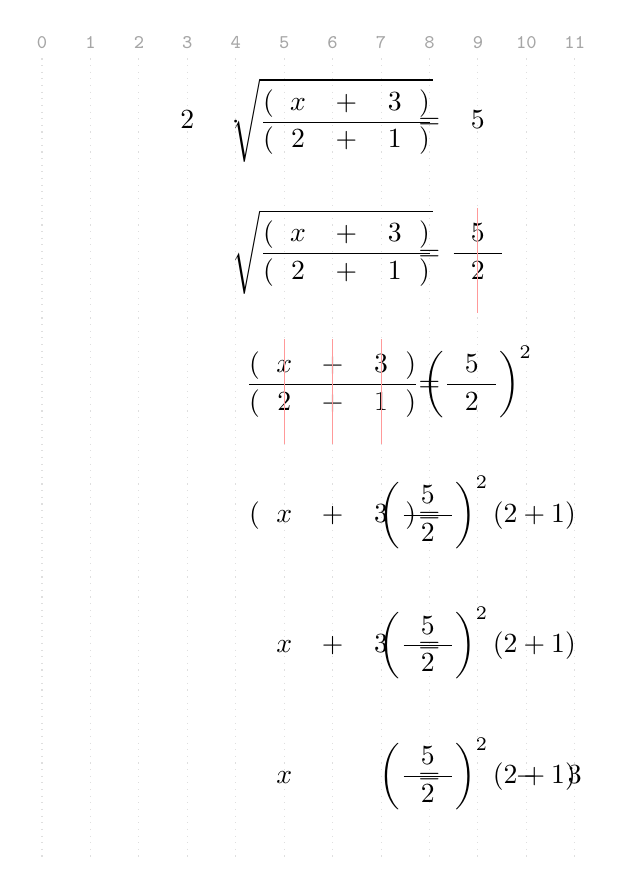
\begin{tikzpicture}[x=1.75em,y=-1em]
\draw[gray!25, dotted] (0,0.35) -- (0,29.330000000000002);
\node[font={\ttfamily\scriptsize}, text=gray!70, anchor=base] at (0,0) {0};
\draw[gray!25, dotted] (1,0.35) -- (1,29.330000000000002);
\node[font={\ttfamily\scriptsize}, text=gray!70, anchor=base] at (1,0) {1};
\draw[gray!25, dotted] (2,0.35) -- (2,29.330000000000002);
\node[font={\ttfamily\scriptsize}, text=gray!70, anchor=base] at (2,0) {2};
\draw[gray!25, dotted] (3,0.35) -- (3,29.330000000000002);
\node[font={\ttfamily\scriptsize}, text=gray!70, anchor=base] at (3,0) {3};
\draw[gray!25, dotted] (4,0.35) -- (4,29.330000000000002);
\node[font={\ttfamily\scriptsize}, text=gray!70, anchor=base] at (4,0) {4};
\draw[gray!25, dotted] (5,0.35) -- (5,29.330000000000002);
\node[font={\ttfamily\scriptsize}, text=gray!70, anchor=base] at (5,0) {5};
\draw[gray!25, dotted] (6,0.35) -- (6,29.330000000000002);
\node[font={\ttfamily\scriptsize}, text=gray!70, anchor=base] at (6,0) {6};
\draw[gray!25, dotted] (7,0.35) -- (7,29.330000000000002);
\node[font={\ttfamily\scriptsize}, text=gray!70, anchor=base] at (7,0) {7};
\draw[gray!25, dotted] (8,0.35) -- (8,29.330000000000002);
\node[font={\ttfamily\scriptsize}, text=gray!70, anchor=base] at (8,0) {8};
\draw[gray!25, dotted] (9,0.35) -- (9,29.330000000000002);
\node[font={\ttfamily\scriptsize}, text=gray!70, anchor=base] at (9,0) {9};
\draw[gray!25, dotted] (10,0.35) -- (10,29.330000000000002);
\node[font={\ttfamily\scriptsize}, text=gray!70, anchor=base] at (10,0) {10};
\draw[gray!25, dotted] (11,0.35) -- (11,29.330000000000002);
\node[font={\ttfamily\scriptsize}, text=gray!70, anchor=base] at (11,0) {11};
\node[anchor=base, inner sep=0pt] at (3,2.9) {$2$};
\node[anchor=base, inner sep=0pt] at (4,2.9) {$\cdot$};
\node[anchor=base, inner sep=0pt] at (6,2.9) {$\sqrt{\displaystyle\frac{\left(\pFourCell{x}\pFourCell{+}\pFourCell{3}\right)}{\left(\pFourCell{2}\pFourCell{+}\pFourCell{1}\right)}}$};
\node[anchor=base, inner sep=0pt] at (8,2.9) {$=$};
\node[anchor=base, inner sep=0pt] at (9,2.9) {$5$};
\node[anchor=base, inner sep=0pt] at (9,7.6499999999999995) {$\displaystyle\frac{\pFourCell{5}}{\pFourCell{2}}$};
\draw[red!40, line width=0.35pt] (9,5.75) -- (9,9.549999999999999);
\node[anchor=base, inner sep=0pt] at (6,7.6499999999999995) {$\sqrt{\displaystyle\frac{\left(\pFourCell{x}\pFourCell{+}\pFourCell{3}\right)}{\left(\pFourCell{2}\pFourCell{+}\pFourCell{1}\right)}}$};
\node[anchor=base, inner sep=0pt] at (8,7.6499999999999995) {$=$};
\node[anchor=base, inner sep=0pt] at (6,12.384999999999998) {$\displaystyle\frac{\left(\pFourCell{x}\pFourCell{+}\pFourCell{3}\right)}{\left(\pFourCell{2}\pFourCell{+}\pFourCell{1}\right)}$};
\draw[red!40, line width=0.35pt] (5,10.499999999999998) -- (5,14.269999999999998);
\draw[red!40, line width=0.35pt] (6,10.499999999999998) -- (6,14.269999999999998);
\draw[red!40, line width=0.35pt] (7,10.499999999999998) -- (7,14.269999999999998);
\node[anchor=base, inner sep=0pt] at (8,12.384999999999998) {$=$};
\node[anchor=base, inner sep=0pt] at (9,12.384999999999998) {$\left(\displaystyle\frac{\pFourCell{5}}{\pFourCell{2}}\right)^{2}$};
\node[anchor=base, inner sep=0pt] at (6,17.104999999999997) {$\left(\pFourCell{x}\pFourCell{+}\pFourCell{3}\right)$};
\node[anchor=base, inner sep=0pt] at (8,17.104999999999997) {$=$};
\node[anchor=base, inner sep=0pt] at (9,17.104999999999997) {$\left(\displaystyle\frac{\pFourCell{5}}{\pFourCell{2}}\right)^{2}\left(2 + 1\right)$};
\node[anchor=base, inner sep=0pt] at (5,21.825) {$x$};
\node[anchor=base, inner sep=0pt] at (6,21.825) {$+$};
\node[anchor=base, inner sep=0pt] at (7,21.825) {$3$};
\node[anchor=base, inner sep=0pt] at (8,21.825) {$=$};
\node[anchor=base, inner sep=0pt] at (9,21.825) {$\left(\displaystyle\frac{\pFourCell{5}}{\pFourCell{2}}\right)^{2}\left(2 + 1\right)$};
\node[anchor=base, inner sep=0pt] at (5,26.545) {$x$};
\node[anchor=base, inner sep=0pt] at (8,26.545) {$=$};
\node[anchor=base, inner sep=0pt] at (9,26.545) {$\left(\displaystyle\frac{\pFourCell{5}}{\pFourCell{2}}\right)^{2}\left(2 + 1\right)$};
\node[anchor=base, inner sep=0pt] at (10,26.545) {$-$};
\node[anchor=base, inner sep=0pt] at (11,26.545) {$3$};
\end{tikzpicture}
\end{center}
\end{document}
